%%%%%%%%%%%%%%%%%%%%%%%%%%%%%%%%%%%%%%%%%
% Short Sectioned Assignment
% LaTeX Template
% Version 1.0 (5/5/12)
%
% This template has been downloaded from:
% http://www.LaTeXTemplates.com
%
% Original author:
% Frits Wenneker (http://www.howtotex.com)
%
% License:
% CC BY-NC-SA 3.0 (http://creativecommons.org/licenses/by-nc-sa/3.0/)
%
%%%%%%%%%%%%%%%%%%%%%%%%%%%%%%%%%%%%%%%%%

%----------------------------------------------------------------------------------------
%	PACKAGES AND OTHER DOCUMENT CONFIGURATIONS
%----------------------------------------------------------------------------------------

\documentclass[paper=a4, fontsize=11pt]{scrartcl} % A4 paper and 11pt font size

\usepackage[T1]{fontenc} % Use 8-bit encoding that has 256 glyphs
\usepackage[ngerman]{babel}
\usepackage{fourier} % Use the Adobe Utopia font for the document - comment this line to return to the LaTeX default
\usepackage{amsmath,amsfonts,amsthm} % Math packages
\usepackage{graphicx}
\usepackage[utf8]{inputenc}
\usepackage{listings}
\usepackage[section]{placeins}
\usepackage{lipsum} % Used for inserting dummy 'Lorem ipsum' text into the template
\usepackage{float}
\usepackage{multicol}

\usepackage{sectsty} % Allows customizing section commands
\allsectionsfont{\centering \normalfont\scshape} % Make all sections centered, the default font and small caps

\usepackage{fancyhdr} % Custom headers and footers
\pagestyle{fancyplain} % Makes all pages in the document conform to the custom headers and footers
\fancyhead{} % No page header - if you want one, create it in the same way as the footers below
\fancyfoot[L]{} % Empty left footer
\fancyfoot[C]{} % Empty center footer
\fancyfoot[R]{\thepage} % Page numbering for right footer
\renewcommand{\headrulewidth}{0pt} % Remove header underlines
\renewcommand{\footrulewidth}{0pt} % Remove footer underlines
\setlength{\headheight}{13.6pt} % Customize the height of the header

\numberwithin{equation}{section} % Number equations within sections (i.e. 1.1, 1.2, 2.1, 2.2 instead of 1, 2, 3, 4)
\numberwithin{figure}{section} % Number figures within sections (i.e. 1.1, 1.2, 2.1, 2.2 instead of 1, 2, 3, 4)
\numberwithin{table}{section} % Number tables within sections (i.e. 1.1, 1.2, 2.1, 2.2 instead of 1, 2, 3, 4)

\setlength\parindent{0pt} % Removes all indentation from paragraphs - comment this line for an assignment with lots of text

%----------------------------------------------------------------------------------------
%	TITLE SECTION
%----------------------------------------------------------------------------------------

\newcommand{\horrule}[1]{\rule{\linewidth}{#1}} % Create horizontal rule command with 1 argument of height

\title{	
\normalfont \normalsize 
\textsc{Karlsruhe Institute of Technology} \\ [25pt] % Your university, school and/or department name(s)
\horrule{0.5pt} \\[0.4cm] % Thin top horizontal rule
\huge Computer Vision for Human-Computer Interaction\\ % The assignment title
\horrule{2pt} \\[0.5cm] % Thick bottom horizontal rule
}

\author{Manuel Lang} % Your name

\date{\normalsize\today} % Today's date or a custom date

\begin{document}

\maketitle % Print the title

%----------------------------------------------------------------------------------------
%	PROBLEM 1
%----------------------------------------------------------------------------------------

\section{Pattern Recognition}

\subsection{Classification}

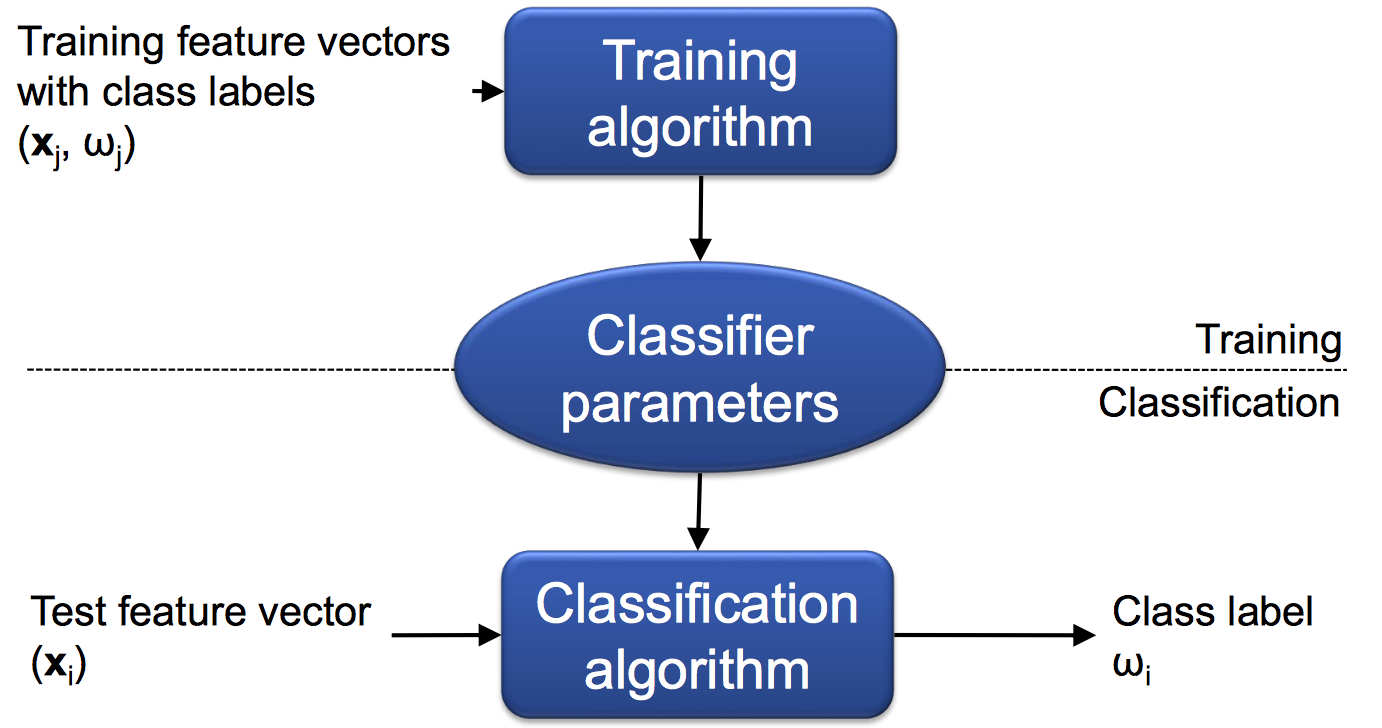
\includegraphics[width=\textwidth]{Klassifizierung}

\subsubsection{Bayesian Classification}

\begin{minipage}{0.45\textwidth}
\begin{itemize}
\item überwacht
\item Featurevektoren $x_1$ bis $x_m$ mit $x_i = <a_1,...a_n>$
\item Vorhersage Klasse $\omega_i$
\item $P(\omega_i | x) = \frac{p(x|\omega_i)P(\omega_i)}{p(x)}$
\end{itemize}
\end{minipage} \hfill
\begin{minipage}{0.5\textwidth}
\begin{figure}[H]
\includegraphics[width=\textwidth]{/Users/Manu/Desktop/bayes.png}
\end{figure}
\end{minipage}

\subsubsection{Gaussian Classification}

\begin{minipage}{0.55\textwidth}
\begin{itemize}
\item Annahme $p(x|\omega_i) \approx N(\mu,\Sigma) = \frac{1}{(2\pi)^{d/2} |\Sigma|^{1/2}} exp[-\frac{1}{2}(x-\mu)^T \Sigma^{-1}(x-\mu)]$
\item Nur $\mu$ und $\Sigma$ müssen geschätzt werden (Maximum Likelihood)
\end{itemize}
\end{minipage} \hfill
\begin{minipage}{0.4\textwidth}
\begin{figure}[H]
\includegraphics[width=\textwidth]{/Users/Manu/Desktop/gauss.png}
\end{figure}
\end{minipage}

\subsubsection{Gaussian Mixture Models (GMMs)}

\begin{minipage}{0.55\textwidth}
\begin{itemize}
\item Gewichtete Summe von mehreren Gaussians
\item $p(x) = \sum\limits_i w_i \frac{1}{(2\pi)^{d/2} |\Sigma|^{1/2}} exp[-\frac{1}{2}(x-\mu)^T \Sigma^{-1}(x-\mu)]$ mit $\sum\limits_i = 1$
\item Gewichte müssen zusätzlich geschätzt werden -> EM
\end{itemize}
\end{minipage} \hfill
\begin{minipage}{0.4\textwidth}
\begin{figure}[H]
\includegraphics[width=\textwidth]{/Users/Manu/Desktop/gmm.png}
\end{figure}
\end{minipage}
\newpage
\subsubsection{Expectation Maximization (EM)}

\begin{itemize}
\item Problem: Zu welchem Gaussian gehört ein Punkt?
\item EM Algorithmus
\begin{itemize}
\item Zufällige Initialisierung der GMM
\item Wiederhole bis Konvergenz
\begin{itemize}
\item Expectation: Berechne die Wahrscheinlichkeit $p_{ij}$, dass ein Punkt $i$ zu einem Gaussian $j$ gehört
\item Maximation: Berechne neue GMM Parameter $p_{ij}$ (Maximum Likelihood)
\end{itemize}
\end{itemize}
\end{itemize}

\subsubsection{Parametrisierte vs nicht-parametrisierte Modelle}

\begin{itemize}
\item Gaussian und GMM sind parametrisiert
\begin{itemize}
\item Wahrscheinlichkeitsverteilung mit Parametern
\item Nur Parameter werden geschätzt
\end{itemize}
\item Methoden die keine spezifische Form der Wahrscheinlichkeitsverteilung vermuten
\begin{itemize}
\item nicht-parametrisiert
\item Parzen windows, k-nearest neighbors
\end{itemize}
\item Parametrisierte Klassifikatoren
\begin{itemize}
\item + weniger Trainingsdaten, da weniger Parameter zu schätzen
\item - funktionieren nur, wenn Model zu Daten passt
\end{itemize}
\item Nicht-parametrisierte Klassifikatoren
\begin{itemize}
\item + Funktionieren für alle Arten von Verteilungen
\item - mehr Trainingsdaten
\end{itemize}
\end{itemize}

\subsubsection{Generative vs diskriminative Modelle}

\begin{itemize}
\item $P(\omega_i)$ und $p(x|\omega_i)$ explizit modelliert $\rightarrow$ generativ: Durch $p(x|\omega_i)$ können neue Samples der Klasse $\omega_i$ generiert werden
\item direktes Modellieren von $P(\omega_i|x)$ oder nur eine Entscheidung $\omega_i$ abhängig von einem Muster $x \rightarrow$ diskriminativ
\item diskriminativ oft leichter zu trainieren
\end{itemize}

\subsubsection{Lineare diskriminative Funktionen}

\begin{itemize}
\item Trenne zwei Klassen $\omega_1, \omega_2$ mit einer linearen Hyperebene $y(x) = w^T x + w_0$
\item Wähle $\omega_1$ für $y(x) > 0$ und $\omega_2$ für $y(x) < 0$ mit dem Normalenvektor $w^T$ der Hyperebene
\item Anwendung: Perzeptron, lineare SVM
\end{itemize}

\subsubsection{Perzeptron}

\begin{minipage}{0.55\textwidth}
\begin{enumerate}
\item Initialisiere $w = 0$ oder zufällig
\item Klassifiziere mit $y(x) = sign(w^Tx)$
\item Falls korrekt, zu 2, sonst $w' = w - \eta \cdot y(x) \cdot x$ 
\item Falls keine Fehler, done, sonst 2
\end{enumerate}
\end{minipage} \hfill
\begin{minipage}{0.4\textwidth}
\begin{figure}[H]
\includegraphics[width=\textwidth]{/Users/Manu/Desktop/perz.png}
\end{figure}
\end{minipage}

\subsubsection{Support Vector Machines}

\begin{minipage}{0.55\textwidth}
\begin{itemize}
\item Hyperebene maximiert den Abstand zwischen positiven und negativen Beispielen
\item Soft-margin: Minimiere $||w||^2 + C \cdot \Sigma \xi_i$ anstatt $||w||^2$ um Abweichungen zuzulassen
\item nicht separierbar $\rightarrow$ Dimension erhöhen, Kernel-Trick
\end{itemize}
\end{minipage} \hfill
\begin{minipage}{0.35\textwidth}
\begin{figure}[H]
\includegraphics[width=\textwidth]{/Users/Manu/Desktop/svm.png}
\end{figure}
\end{minipage}

\subsubsection{k-nearest-neighbors (KNN)}

\begin{minipage}{0.55\textwidth}
\begin{itemize}
\item Betrachte k nächste Trainingsamples und verwende meist vorkommendes Label
\item Model beinhaltet alle Trainingsdaten
\begin{itemize}
\item + kein Informationsverlust
\item - viel Daten (Performanz)
\item Distanz wird für jeden Testdatensatz neu berechnet
\end{itemize}
\item Distanzmetrik benötigt
\begin{itemize}
\item Wichtiger Parameter
\item $L_1$, $L_2$, $L_\infty$, Mahalanobis, ...
\item Wird abhängig von Problemstellung verwendet
\end{itemize}
\end{itemize}
\end{minipage} \hfill
\begin{minipage}{0.4\textwidth}
\begin{figure}[H]
\includegraphics[width=\textwidth]{/Users/Manu/Desktop/knn.png}
\end{figure}
\end{minipage}

\subsection{Clustering}

\begin{minipage}{0.5\textwidth}
\begin{itemize}
\item Nur Datensätze, keine Labels
\item Strukturen werden erkannt
\end{itemize}
\end{minipage} \hfill
\begin{minipage}{0.45\textwidth}
\begin{figure}[H]
\includegraphics[width=\textwidth]{/Users/Manu/Desktop/cluster.png}
\end{figure}
\end{minipage}

\subsubsection{K-means}

\begin{itemize}
\item Zufällige Initialisierung von $k$ Clustern
\item Wiederhole bis Konvergenz
\begin{itemize}
\item Datenpunkte zu nächstem Clusterzentrum
\item Berechne neue Clusterzentren in der Mitte der zugewiesenen Punkte
\end{itemize}
\item + einfach und effizient
\item - Anzahl $k$ muss vorgegeben werden
\item - Ergebnis abhängig von Initialisierung
\item - funktioniert nicht für verschiedene Clustertypen (runde, überlappend)
\item ähnlich zu EM, benutzt aber feste Zuweisungen anstatt probabilistischen (EM)
\item EM kann für Clustering verwendet werden
\end{itemize}

\subsubsection{Agglomerative Hierarchical Clustering}

\begin{minipage}{0.5\textwidth}
\begin{itemize}
\item Jeder Punkt ist zu Beginn Cluster
\item Vereine die zwei nächsten Cluster
\item Verschiedene Distanzmaße möglich (min,max,avg,mean)
\item Ergebnis ist Baumstruktur (Dendrogram)
\end{itemize}
\end{minipage} \hfill
\begin{minipage}{0.45\textwidth}
\begin{figure}[H]
\includegraphics[width=\textwidth]{/Users/Manu/Desktop/ahc.png}
\end{figure}
\end{minipage}

\subsubsection{\glqq Curse of dimensionality\grqq}

\begin{itemize}
\item Featurevektoren haben oft sehr hohe Dimensionalität
\item Operationen der linearen Algebra nicht mehr anwendbar
\item Klassifikatoren arbeiten besser in niedriger Dimensionalität
\item Entstehende Probleme bei hoher Dimensionalität $\rightarrow$ \glqq Curse of dimensionality\grqq
\end{itemize}

\subsection{Dimensionality reduction}

\subsubsection{PCA}

\begin{minipage}{0.6\textwidth}
\begin{itemize}
\item Finde Richtungsvektoren, die den Fehlerschnitt minimieren, durch Kovarianzmatrix
\item Projiziere auf den durch diese Vektoren aufgespannten Raum
\item Projiziere auf $K$ Richtungsvektoren um die Dimensionalität zu reduzieren
\end{itemize}
\end{minipage} \hfill
\begin{minipage}{0.35\textwidth}
\begin{figure}[H]
\includegraphics[width=\textwidth]{/Users/Manu/Desktop/pca.png}
\end{figure}
\end{minipage}

\subsubsection{LDA}

\begin{minipage}{0.6\textwidth}
\begin{itemize}
\item TODO
\end{itemize}
\end{minipage} \hfill
\begin{minipage}{0.35\textwidth}
\begin{figure}[H]
\includegraphics[width=\textwidth]{/Users/Manu/Desktop/lda.png}
\end{figure}
\end{minipage}

\section{Gesichtsdetektion}

\subsection{Wieso Gesichtserkennung?}

\begin{itemize}
\item Personenidentifizierung
\item Erkennung von Emotionen/Posen
\item Mund als Quelle der Sprachen
\item Lippenlesen
\item Absichtserkennung
\item Erkennung von Alter, Geschlecht, Hautfarbe
\item Ansatz: Hautfarbe hat konsistente Farbwerte
\end{itemize}

\subsection{Farbräume}

\begin{itemize}
\item RGB (Rot, Grün, Blau)
\item HSV/HSI (Hue, Saturation, Value/Intensity)
\item Y-Klasse: YCbCr (Videos), YIQ (NTSC), YUV (PAL): Trennung von Helligkeit (Y) und Chrominanz
\end{itemize}

\subsection{Modellierung von Hautfarbe}

\begin{itemize}
\item nicht-parametrisiert (Histogramme)
\item parametrisierte (Gauss, Gauss-Mixturen)
\item Grenzen lernen (diskriminative Modelle, ANN, SVM, ...)
\end{itemize}

\subsection{Histogram Backprojection}

\begin{itemize}
\item einfacher und schneller Ansatz
\item Jeder Pixel in der Rückprojektion wird auf das Histrogram-Bin des Farbwerts gesetzt
\end{itemize}

\subsection{Histogram Matching}

\begin{itemize}
\item Backprojection gut bei monomodaler Farbverteilung, aber schlecht bei bunten Zielen
\item Lösung: Histrogramm innerhalb des Suchfensters wird mit Ziel verglichen
\item Verschiedene Distanzmetriken (Battacharya Distanz, Histogram intersection, Earth-movers distance, ...)
\end{itemize}

\subsection{Vergleich Histrogram Backprojection vs Histogram Matching}

\begin{minipage}{0.45\textwidth}
\begin{center}
Histogram Backprojection
\end{center}
\begin{itemize}
\item Vergleicht Farbe eines einzelnen Pixels mit Farbmodell
\item schnell und einfach
\item nur gut bei monomodaler Verteilung
\item genügt für Klassifizierung von Hautfarbe
\end{itemize}
\end{minipage} \hfill
\begin{minipage}{0.45\textwidth}
\begin{center}
Histogram Matching
\end{center}
\begin{itemize}
\item Vergleicht Farbhistrogramm des Bildes mit Farbmodell
\item bessere Ergebnisse
\item anwendbar für multimodale Verteilung
\item teure Berechnungen
\end{itemize}
\end{minipage}

\subsection{Gaussian Density Models}

\begin{itemize}
\item Annahme: Verteilung der Hautfarben $p(x)$ hat die Form einer parametrischen Funktion
\item Gauss-Funktion $G(x, \mu, C)$: $p(x|skin) = G(x; \mu, C) = (2\pi)^{-d/2} |C|^{-1/2} exp\{-1/2(x-\mu)^T C^{-1} (x-\mu)\}$
\item Mittel $\mu$ und Kovarianz-Matrix $C$ werden aus Trainingsdatensatz von Hautfarben $S = \{s_1,x_2,...,x_N\}$ geschätzt. $\mu = E\{x\}$, $C = E\{(x-\mu)(x-\mu)\}$
\item Klassifizierung $p(x|skin) > \theta$ oder $p(x|skin) > p(x|non-skin)$
\end{itemize}

\subsection{Mixture of Gaussians Models}

\begin{itemize}
\item Ein Gaussian kann zu wenig sein, um eine Hautfarben-Verteilung genügend zu beschreiben (z.B. HS-Raum): $p(x) = \sum\limits_{i=1}^K \pi_i G(x, \mu_i, C_i)$
\item Parameterset $\Phi$ kann durch EM Algorithmus geschätzt werden: $L = log \prod\limits_{i=1}^N p(x_i|\Phi)$
\item Klassifizierung $p(x|skin) > \theta$ oder $p(x|skin) > p(x|non-skin)$
\end{itemize}

\subsection{Bayes Classifier}

\begin{itemize}
\item minimale Kosten
\item Klassifikation $P(Skin|x) > P(Non-Skin|x)$
\item Entscheidungsregel: $\frac{p(x|Skin)}{p(x|Non-Skin)} \ge \frac{P(Non-Skin)}{P(Skin)}$
\item Die Klassenbedingungen $p(x|\omega)$ können über die korrespondierenden Histogramme geschätzt werden: $p(x|\omega_i) = h_i(x) / \sum\limits_x h_i(x)$, $h_i(x)$ - Anzahl der Pixel der Klasse $\omega_i$ mit dem Wert (x)
\end{itemize}

\subsection{Diskriminative Modelle / Klassifikatoren}

\begin{itemize}
\item Künstliche Neuronale Netze (ANNs)
\item Support Vector Machines
\item ...
\end{itemize}

\subsection{Performanz-Metriken}

\begin{itemize}
\item ROC (Receiver-Operating-Characteristic)\\
\begin{minipage}{0.6\textwidth}
\begin{itemize}
\item Anwendung: Klassifiation
\item Trade-off zwischen true positive und false positive
\item true positive rate = TP / Pos = TP / (TP+FN)
\item false positive rate = FP / Neg = FP / FP + TN
\end{itemize}
\end{minipage} \hfill
\begin{minipage}{0.35\textwidth}
\begin{figure}[H]
\includegraphics[width=\textwidth]{/Users/Manu/Desktop/roc.png}
\end{figure}
\end{minipage}
\item RPC (Recall-Precision-Curve)
\item DET (Detection Error Trade-Off)
\end{itemize}

\subsection{Morphologische Operatoren}

\begin{itemize}
\item Erosion\\
\begin{minipage}{0.5\textwidth}
\begin{itemize}
\item entfernt Pixel an Ecken von Objekten
\item setzt Pixelwerte auf das Minimum der umliegenden Pixel
\end{itemize}
\end{minipage} \hfill
\begin{minipage}{0.45\textwidth}
\begin{figure}[H]
\includegraphics[width=\textwidth]{/Users/Manu/Desktop/ero.png}
\end{figure}
\end{minipage}
\item Dilatation\\
\begin{minipage}{0.5\textwidth}
\begin{itemize}
\item fügt Pixel an Ecken von Objekten ein
\item setzt Pixelwerte auf das Maximum der umliegenden Pixel
\end{itemize}
\end{minipage} \hfill
\begin{minipage}{0.45\textwidth}
\begin{figure}[H]
\includegraphics[width=\textwidth]{/Users/Manu/Desktop/dil.png}
\end{figure}
\end{minipage}
\begin{minipage}{0.5\textwidth}
\item Opening
\begin{itemize}
\item erst Erosion, dann Dilatation
\item Glätten, Lücken einfügen, Outliers eliminieren
\end{itemize}
\item Closing
\begin{itemize}
\item erst Dilatation, dann Erosion
\item Glätte innere Ecken, verbinde kleine Distanzen, fülle unerwünschte Löcher
\end{itemize}
\end{minipage} \hfill
\begin{minipage}{0.2\textwidth}
\begin{figure}[H]
\includegraphics[width=\textwidth]{/Users/Manu/Desktop/ope.png}
\end{figure}
\end{minipage} \hfill
\begin{minipage}{0.2\textwidth}
\begin{figure}[H]
\includegraphics[width=\textwidth]{/Users/Manu/Desktop/clo.png}
\end{figure}
\end{minipage}
\end{itemize}

\subsection{Gesichtsdetektion mit neuronalen Netzen}

\begin{itemize}
\item Ansatz: Verwende neuronales Netz um aufrechte frontale Gesichter zu erkennen
\item Input: 20x20 Pixel Bildregion
\item Bereich -1 (kein Gesicht) bis 1 (Gesicht)
\item Filter auf gesamtes Bild angewendet
\item Bild wird skaliert, um Gesichter mit verschiedenen Größen zu erkennen
\item Training
\begin{itemize}
\item 1050 normalisierte Bilder von Gesichtern
\item 15 Bilder von rotierten und skalierten Gesichtsbildern
\item 1000 zufällig ausgewählte Bilder ohne Gesichter
\end{itemize}
\item Vorverarbeitung
\begin{itemize}
\item Beleuchtungskorrektur
\item Skalieren auf einheitliche Größe
\end{itemize}
\begin{minipage}{0.5\textwidth}
\item Histogram equalization (Histogramspreizung)
\begin{itemize}
\item definiert Mapping von Graufwerten p auf Grauwerte q, sodass die Grauwerte q einheitlich verteilt werden
\item erweitert den Bereich der Graustufen (erhöht Kontrast)
\item bildet Eingabebilder so ab, dass sie ähnliche Intensitätsverteilungen haben
\end{itemize}
\end{minipage} \hfill
\begin{minipage}{0.45\textwidth}
\begin{figure}[H]
\includegraphics[width=\textwidth]{/Users/Manu/Desktop/hiseq.png}
\end{figure}
\end{minipage}
\item Ausgabe eines KNNs definiert einen Filter für Gesichter
\item Suche: Wende Suchfenster auf Eingabebild an, wende auf Suchfenster KNN an, Eingabebild muss skaliert werden um Gesichter mit unterschiedlicher Größe zu erkennen
\item Nachverarbeitung: Rauschreduktion, kombinierende sich überschneidende Ergebnisse
\item Geschwindigkeits-Optimierung: erhöhe Schrittweite, mache ANN flexibler ggü Translationen, hierarchische Suche
\end{itemize}

\subsection{Feature-basierte Gesichtsdetektion}

\begin{itemize}
\item Erkennung mit (Haar-Like) Features statt Pixeln: Features können umgebungsabhängiges Wissen beinhalten, was schwierig zu lernen ist, schneller als Pixel-basierte Ansätze, skalierungs-invariant
\item Robuste Echtzeiterkennung von Featuren (Gesichter), Integralbildern (um Feature zu bestimmen), schwachen Klassifikatoren (Kaskaden) und Trainieren der Kaskaden
\item Anwendung von Suchfenstern (z.B. 24x24px), viele Features können ausgelesen werden, daher können nicht alle Features bestimmt werden
\item Integral Image: $ii(x,y) = \sum\limits_{x' \le x, y' \le y} i(x',y')$
\item Bestimmung aller Features dauert nachwievor zu lange, nur entscheidende Features sollen gelernt werden
\end{itemize}

\subsubsection{AdaBoost}

\begin{minipage}{0.6\textwidth}
\begin{itemize}
\item Ziel: Erhöhen der Klassifizierungsergebnisse von einfachen Algorithmen (z.B. Perzeptron)
\item Variante davon wird verwendet um Features auszuwählen und den Klassifikator zu trainieren
\item kombiniert mehrere schwache Klassifikatoren um einen starken zu bilden
\item schwacher Klassifikator $h$ mit Genauigkeit geringfügig besser als Zufall
\item kombiniere schwache Klassifikatoren $h_i \in \{-1,1\}$ linear zu einem starken Klassifikator $H = sign \sum\limits_{i=1}^N w_i h_i$
\item Viola \& Jones: Schwache Klassifikatoren $h_j(x)$ bestehen aus Featuren $f_j$, einem Threshold $\theta_j$ und einer Polarität $p_j$, die die Richtung des $sign$ indiziert
\begin{equation*}
   h_j(x) =
   \begin{cases}
     1 & \text{f"ur } p_j f_j(x) \textless p_j \theta_j \\
     0 & \text{sonst}
   \end{cases}
\end{equation*}
\item selektiert die schwachen Klassifikatoren mit der geringsten Fehlerrate
\item effizient für wenig gute Features mit hoher Varianz
\end{itemize}
\end{minipage} \hfill
\begin{minipage}{0.35\textwidth}
\begin{figure}[H]
\includegraphics[width=\textwidth]{/Users/Manu/Desktop/ada.png}
\end{figure}
\end{minipage}

\subsubsection{Classifier Cascade}

\begin{minipage}{0.5\textwidth}
\begin{itemize}
\item nicht alle Fenster enthalten Gesichter, Klassifikator muss aber trotzdem für alle angewandt werden
\item Ansatz: Kaskade von Klassifaktoren
\begin{itemize}
\item Jeder weitere Klassifikator ist genauer: erste Schicht entdeckt alle positiven Beispiele, aber enthält viele falsche, zweite fokussiert auf false positive des ersten Layers, ...
\item Fenster ohne Gesichter werden schnell aussortiert, Gesichter werden bis zum Ende weitergereicht
\end{itemize}
\end{itemize}
\end{minipage} \hfill
\begin{minipage}{0.45\textwidth}
\begin{figure}[H]
\includegraphics[width=\textwidth]{/Users/Manu/Desktop/cascade.png}
\end{figure}
\end{minipage}

\subsubsection{Cascade Training}

\begin{itemize}
\item senkt false positive Rate in jeder Schicht (allgemein weniger erkannte Gesichter)
\item In jeder Schicht wird Ziel auf minimale Reduktion gesetzt. Ziel wird erreicht, indem weitere Features zur Schicht hinzugefügt werden.
\item Schichten werden hinzugefügt, bis Ziel der Falschklassifikation erreicht wird
\item Jede Schicht wird komplexer und beinhaltet mehr Features
\end{itemize}

\subsubsection{Rotierte Bilder}

\begin{figure}[H]
\includegraphics[width=\textwidth]{/Users/Manu/Desktop/rot.png}
\end{figure}

\subsubsection{Zusammenfassung Viola \& Jones}

\begin{itemize}
\item Ansatz ist 15x schneller als bisherige Ansätze
\item Anwendung auf verschiedene Objekte möglich
\item Einfluss auf eine Vielzahl anderer Aufgaben
\item entdeckt mehrere Gesichter in Bildern
\item robust gegen Illuminanz
\end{itemize}

\section{Gesichtsidentifikation}

\subsection{Herausforderungen}

\begin{itemize}
\item abweichende Beleuchtung
\item abweichender Blickwinkel (frontal, nicht-frontal)
\item Occlusion (Sonnenbrille, Hut, Bart, Make-up)
\item Gesichtsausdrücke
\item Alter
\end{itemize}

\subsection{Closed Set vs. Open Set Identification}

\begin{itemize}
\item Closed-Set: Wer ist die Person?
\item Open-Set: Ist Person in Daten? Wenn ja, wer?
\begin{enumerate}
\item False accept: Person nicht in Daten, aber so erkannt
\item False reject: Person in Daten, aber nicht erkennt
\item False classify: Person ist in Daten, so erkannt, aber die falsche Person zugeordnet
\end{enumerate}
\end{itemize}

\subsection{Feature-basierte Gesichtsidentifikation}

\begin{minipage}{0.65\textwidth}
\begin{itemize}
\item Dicke der Augenbrauen
\item Position von Augen, Nase und Mund
\item Breite der Nase
\item Mund-Höhe und -Breite
\item 11 Kanten zwischen Mund und Kinn
\item Gesichtsbreite auf Nasenhöhe
\end{itemize}
\end{minipage} \hfill
\begin{minipage}{0.3\textwidth}
\begin{figure}[H]
\includegraphics[width=\textwidth]{/Users/Manu/Desktop/fea.png}
\end{figure}
\end{minipage}

\subsection{Appearance-basierte Gesichtsidentifikation}

\begin{minipage}{0.65\textwidth}
\begin{itemize}
\item entweder holistisch (gesamtes Gesicht als Eingabe)
\item oder lokal/fiduziell (Berechnung von Gesichtsfeaturen wie Augen, Mund, etc. getrennt)
\end{itemize}
\end{minipage} \hfill
\begin{minipage}{0.3\textwidth}
\begin{figure}[H]
\includegraphics[width=\textwidth]{/Users/Manu/Desktop/app.png}
\end{figure}
\end{minipage}

\subsection{Eigenfaces}

\begin{minipage}{0.65\textwidth}
\begin{itemize}
\item Gesichtsbild definiert einen Punkt im hochdimensionalen Bildraum
\item verschiedene Gesichtsbilder haben eine Reihe von Gemeinsamkeiten
\item Gesichtsbilder können in einem eher geringen Unterraum beschrieben werden
\item Abbildung des Gesichtsbild in einen Unterraum und berechne Ähnlichkeit
\item Verwendung von PCA: Analysierte Komponenten werden Eigenfaces genannt und spannen den \glqq face space\grqq\ auf
\item Probleme:
\begin{itemize}
\item Eigenfaces unterscheides nicht zwischen Shape und Appearance -> ASM/AAM
\item PCA verwendet keine Klasseninformationen
\end{itemize}
\end{itemize}
\end{minipage} \hfill
\begin{minipage}{0.3\textwidth}
\begin{figure}[H]
\includegraphics[width=\textwidth]{/Users/Manu/Desktop/eigen.png}
\end{figure}
\end{minipage}

\subsection{Fisherfaces}

\begin{minipage}{0.65\textwidth}
\begin{itemize}
\item verwendet LDA (Linear Discriminant Analysis)
\item wahrt Separierbarkeit der Klassen
\item Maximiert Verhältnis von Streuung zwischen Klassen zu Streuung innerhalb von Klassen\\ 
$W_{fId} = arg\max\limits_W \frac{|W^T S_B W|}{|W^T S_W W|}$
\item Streuung zwischen Klassen
$S_B = \sum\limits_{i=1}^c |x_i| (\mu_i - \mu) (\mu_i-\mu)^T$
\item Streuung innerhalb von Klassen
$S_W = \sum\limits_{i=1}^c \sum\limits_{x_k \in X_i} (x_k - \mu_i) (x_k - \mu_i)^T$
\item mit $c$: Anzahl der Klassen, $\mu_i$: Durchschnitt der Klasse $X_i$, $|X_i|$: Anzahl der Samples von $X_i$
\item Fisherfaces werden unabhängig von Unterschieden innerhalb von Klassen (Beleuchtung, Gesichtsausdrücke)
\end{itemize}
\end{minipage} \hfill
\begin{minipage}{0.3\textwidth}
\begin{figure}[H]
\includegraphics[width=\textwidth]{/Users/Manu/Desktop/fisher.png}
\end{figure}
\end{minipage}

\subsection{Problem: Matching mit verschiedenen Posen}

\begin{itemize}
\item Problem: verschiedene Blickrichtung, Kopforientierung
\item verschlechtert Erkennung
\item Ansätze: Pose-Normalization, 2D Pose Modelle, 2D+3D Modelle, 3D face Model fitting
\end{itemize}

\subsection{Pose-Normalization}

\begin{minipage}{0.65\textwidth}
\begin{itemize}
\item Alignment mit Augenpunkten ist nicht ausreichend
\item Idee
\begin{itemize}
\item Detektiere mehrere Gesichtsfeatures (Meshes)
\item nutze Mesh um Gesicht zu normalisieren
\end{itemize}
\item Rechts: 2d Active Appearance Models
\begin{itemize}
\item basiert auf Textur und Forum (parametrisiert)
\item Inverse compositional (IC) Algorithmus
\end{itemize}
\item Modell kann verwendet werden, um Bild in frontale Pose zu transformieren
\end{itemize}
\end{minipage} \hfill
\begin{minipage}{0.2\textwidth}
\begin{figure}[H]
\includegraphics[width=\textwidth]{/Users/Manu/Desktop/2daam.png}
\end{figure}
\end{minipage}

\subsection{Face Recognition Based on Fitting a 3D Morphable Model}

\begin{minipage}{0.55\textwidth}
\begin{itemize}
\item Methode zur Umgehung von Variationen in Pose und Beleuchtung
\item Simuliert die Bild-Entstehung im 3D Raum
\item Schätzt 3D Shape und Textur von Gesichtern aus einem Bild durch Anwenden eines morphable models von 3D Gesichtern auf das Bild
\item Gesichter sind Modell-Paramater für 3D Shape und Textur (Shape: $S = \sum\limits_{i=1}^m a_iS_i$, Textur: $T = \sum\limits_{i=1}^m b_iT_i$)
\end{itemize}
\end{minipage} \hfill
\begin{minipage}{0.4\textwidth}
\begin{figure}[H]
\includegraphics[width=\textwidth]{/Users/Manu/Desktop/3dmm.png}
\end{figure}
\end{minipage}

\subsection{Local feature based Face Recognition}

\subsubsection{Gabor Filter}

\begin{minipage}{0.55\textwidth}
\begin{itemize}
\item 2D Sinuskurven moduliert durch Gaussglocke
\item $g(x,y, \lambda, \theta, \psi, \sigma, \gamma) = exp(-\frac{x'^2 + \gamma^2 y'^2}{2 \sigma^2}) exp (i(2\pi \frac{x'}{\lambda} + \psi)) $
\item Gabor Wavelet Transformation (GTW)
\begin{itemize}
\item $O_{u,v}(x,y) = I(x,y) * \psi_{u,v}(x,y)$
\item Typischerweise werden mehrere Skalierungsfaktoren $u$ und Orientierungen $v$ verwendet
\item $O_{u,v}(x,y)$ wird hochdimensionaler Vektor
\item Dimensionsreduzierung (z.B. PCA)
\end{itemize}
\end{itemize}
\end{minipage} \hfill
\begin{minipage}{0.4\textwidth}
\begin{figure}[H]
\includegraphics[width=\textwidth]{/Users/Manu/Desktop/gabor.png}
\end{figure}
\end{minipage}

\subsubsection{Local Binary Patterns (LBP)}

\begin{minipage}{0.65\textwidth}
\begin{itemize}
\item Teile Bild in Zellen
\item Vergleiche jeden Pixel mit seinen Nachbarn
\item Pixelwert > Threshold ? 1 : 0, liefert Binärzahl
\item Konvertiere binär zu dezimal
\item Berechne Histrogram über die Zelle
\item Nutze Histogramm für Klassifikation (z.B. SVM/Histrogramm-Entfernung)
\end{itemize}
\end{minipage} \hfill
\begin{minipage}{0.3\textwidth}
\begin{figure}[H]
\includegraphics[width=\textwidth]{/Users/Manu/Desktop/lbp.png}
\end{figure}
\end{minipage}

\subsubsection{Dense features}

Features werden dicht berechnet, z.B. Filter auf Bild in mehreren Skalierungen.\\ 
Problem: Hohe Dimensionalität\\ 
Ansätze: Bag of Visual Words, Fisher encoding

\subsubsection{Fisher Vector Encoding}

\begin{itemize}
\item kompakte Repräsentation von Featurevektoren
\item parametrisiertes generatives Model (z.B. GMM)
\end{itemize}

\subsubsection{Discrete Cosine Transform (DCT)}

\subsubsection{SIFT}

\subsubsection{Bag of Visual Words (BoVW)}

\subsection{Face Recognition mit Deep Learning}

\subsubsection{DeepFace (Facebook)}

\begin{itemize}
\item Ansatz: Lerne ein tiefes (7 Schichten) NN (20 Millionen Parameter) mit 4 Millionen Personen direkt auf RGB-Pixeln
\item Alignment: 6 Gesichtspunkte für 2D warp, 67 Punkte für 3D Modell, transformiere Gesicht in Frontal-Pose als Input für NN
\item k-way softmax -> Verteilung über Klassenlabels
\item Ziel: Maximiere Wahrscheinlichkeit für korrekte Klasse
\end{itemize}

\includegraphics[width=\textwidth]{/Users/Manu/Desktop/fb.png}

\subsubsection{FaceNet (Google)}

\begin{itemize}
\item Mappe Bilder in kompakten euklidischen Raum, sodass Entfernung $\approx$ Ähnlichkeit der Gesichter
\item Finde $f(x) \in \mathbb{R}^d$ sodass:\\ 
$d^2(f(x_1), f(x_2)) \rightarrow$ klein für gleiche Identität $x_1$ und $x_2$\\ 
$d^2(f(x_1), f(x_2)) \rightarrow$ groß für verschiedene Identitäten 
\item Ansatz: Convolutional Neural Networks optimieren Einbettung, Triplet-based loss function -> training\\ 
\includegraphics[width=\textwidth]{/Users/Manu/Desktop/go1.png}
\end{itemize}

\subsubsection{Deep Face recognition (Oxford)}

\begin{itemize}
\item sehr tiefes Netzwerk
\item sehr wenig conv. Kernels
\end{itemize}

\section{Facial Feature Detection}

\begin{itemize}
\item Teile von Gesichtsregionen, die entscheidende Informationen beinhalten, bspw. Augen, Augenbrauen, Nase, Mund (auch Landmarks genannt)
\item Die Detektion dieser spezifischen Gesichtsbereiche wird Facial Feature Detection genannt
\end{itemize}


\begin{minipage}{0.65\textwidth}
\subsection{Anwendungen}

\begin{itemize}
\item Gesichtserkennung: Geometrische Features zur Identifikation, Facial Features zur Normalisierung bei appearance based models, nötig für lokale / modulare Ansätze
\item model-based head post estimation: Pose von 2D zu 3D
\item Blick tracking: Lokalisierung der Augen
\item facial expression recognition: Bewegung von Augen, Augenbrauen und Mund um Emotionen zu analysieren
\item Modellierung von Alter: Gesichtszüge/-Strukturen unterscheiden sich im Alter
\end{itemize}
\end{minipage} \hfill
\begin{minipage}{0.35\textwidth}

\subsection{Probleme}

\begin{itemize}
\item verschiedene Personen
\item verschiedene Expressionen
\item verschiedene Kopfdrehungen
\item verschiedene Skalierungen
\item Beleuchtung
\item Occlusion
\end{itemize}
\end{minipage}

\subsection{Statistical Appearance Models}

\begin{itemize}
\item Idee: Verwendung von priori Wissen (Modellen um die Komplexität der Aufgabe zu reduzieren)
\item muss mit Varianz umgehen können (-> deformierbare Modelle)
\item verwende statisische Modelle von Shape und Texturen um Landmarken zu finden
\end{itemize}

Appearance Models
\begin{itemize}
\item repräsentieren Textur und Form
\item statistischen Modell aus Trainingsdaten gelernt
\item Modellieren der Form-Varianz $x = [x_1,y_1,x_2,y_2,...,x_n,y_n]^T$ ergibt Modell $x \approx \bar{x} + P_s b_s$
\item Modellieren der Intensitäts-Varianz $h = [g_1,g_2,...,g_k]^T$ ergibt Modell $h \approx \bar{h} + P_i b_i$
\item Konstruiere Shape-Model mit PCA ($x = \bar{x} + P_s b_s)$
\item Konstruiere Texturmodell an jedem Punkt (image warping, texture wrapping) ($g = \bar{g} + P_g b_g)$
\item Modelliere die Verbindung zwischen Shape und Grauwerten (Textur)
\end{itemize}

\subsection{Active Shape Models}

\begin{itemize}
\item Geg. grobe Startposition, erstelle eine Instanz von $X$ mit Shape $b$, Translation $T=(X_t,Y_t)$, Skalierung $s$ und Rotation $\theta$
\item Iterativer Ansatz
\begin{enumerate}
\item Untersuche Bildbereich im Bereich von $X_i$ um das beste Match für den Punkt $X'_i$ zu finden
\item Aktualisiere Parameter ($b,T,s,\theta)$ für den neuen Punkt
\item Wiederhole bis Konvergenz
\end{enumerate}
\item Praxis: Suche entlang der Normalen des Profils\\ 
\includegraphics[width=0.6\textwidth]{/Users/Manu/Desktop/assuche.png}
\end{itemize}

\subsection{Active Appearance Models}

\begin{itemize}
\item Nachteile von ASM: verwendet hauptsächlich Form und weniger Textur
\item Ansatz AAM: Optimiere Parameter (minimiere die Differenz zwischen künstlichem Bild und Ziel) mit Gradientenabstieg\\
\includegraphics[width=0.9\textwidth]{/Users/Manu/Desktop/aam.png}
\end{itemize}

\subsubsection{ASM vs AAM}

\begin{itemize}
\item ASM
\begin{itemize}
\item Versucht ein Set von Modellpunkten auf ein Image durch ein statistischen Shape-Modell zu matchen
\item verwendet iteratives Vorgehen (Variante von EM)
\item Lokale Suche zur Bestimmung des besten Landmarks
\item Anschließend aktualisieren der Parameter um die Modellpunkte näher an die neuen Punkte des Bildes zu transformieren
\end{itemize}
\item AAMs matchen sowohl Position der Modellpunkte als auch Repräsentation der Textur des Objekts auf ein Bild (verwendet Differenz des aktuell erzeugten Bildes und des Ziels um die Parameter zu aktualisieren, typischerweise weniger Landmarks)
\item statistische appearance models liefern eine kompakte Repräsentation
\item können verschiedene Identitäten, Gesichtsausdrücke, Vorkomnisse etc modeliieren
\item Gelabelte Bilder benötigt
\item sehr rechenaufwendig, jedoch existieren Verfahren zur Beschleunigung (Multi-resolution search, constrained aam search, inverse compositional AAMs (CMU))
\item Anwendung: Detektion von fiducial points, face recognition, pose estimation, facial expression analysis, audio-visual speech recognition
\end{itemize}

\subsection{Conditional Random Forests}

\includegraphics[width=0.9\textwidth]{/Users/Manu/Desktop/crf.png}

\subsubsection{Regression trees}

\begin{minipage}{0.65\textwidth}
\begin{itemize}
\item Aufbau wie Entscheidungsbaum zur Klassifizierung
\item Wurzeln: Entscheidung als Vergleich von Zahlen
\item Blätter: Zahlen oder Zahlenvektoren
\end{itemize}
\end{minipage} \hfill
\begin{minipage}{0.3\textwidth}
\begin{figure}[H]
\includegraphics[width=\textwidth]{/Users/Manu/Desktop/reg.png}
\end{figure}
\end{minipage}

\subsubsection{Random regression forests}

\begin{minipage}{0.55\textwidth}
\begin{itemize}
\item 1 Wald = viele Bäume
\item Random, da verschiedene Bäume auf einem random Subset der Trainingsdaten trainiert werden, nach dem Training werden die Vorhersagen der verschiedenen Bäume gemittelt (von allen regression trees)
\end{itemize}
\end{minipage} \hfill
\begin{minipage}{0.4\textwidth}
\begin{figure}[H]
\includegraphics[width=\textwidth]{/Users/Manu/Desktop/rrf.png}
\end{figure}
\end{minipage}

\subsubsection{Facial feature detection with Conditional Regression Forests}

\begin{itemize}
\item State of the art!!!
\item trainiere verschiedene Sets von Bäumen für verschiedene Posen
\item Wurzelknoten akkumulieren die Votes für die verschiedenen facial difucial points auf
\item jeder Baum wird mit einem random ausgewählten Set von Bildern trainiert
\item extrahiert Patches in jedem Bild
\item Trainingsziel: akkumuliere Wahrscheinlichkeit für einen Featurepunkt $C_n$ gegeben einem Patch $P$ im Blattknoten
\item Training
\begin{itemize}
\item Berechne Wahrscheinlichkeit für konkrete Kopfpose
\item Teile das Trainingsset für jede Pose
\item Trainiere regression forest für jedes Subset
\end{itemize}
\item Testen
\begin{itemize}
\item Schätze Wahrscheinlichkeiten für jede Kopfpose
\item Wähle Bäume von verschiedenen regression forests
\item Schätze die density Funktion für alle facial feature points
\item Clustering über alle Featurekandidaten für einen gegeben facial feature point
\end{itemize}
\end{itemize}

\section{Facial Expression Analysis}

6 grundlegende Emotionen (Ekman)\\
\includegraphics[width=\textwidth]{/Users/Manu/Desktop/emo.png}

\subsection{Vorgehensweise}

\includegraphics[width=0.8\textwidth]{/Users/Manu/Desktop/feaab.png}

\subsection{Facial Action Coding System (FACS)}

\begin{itemize}
\item human-observer basiertes System designt um feine Änderungen in facial features zu erkennen
\item Beim Betrachten von in SlowMo aufgenommenem facial behavior kann der trainierte observer alle möglich Gesichtsausdrücke in FACS abbilden
\item  Diese Gesichtsausdrücke werden als action units (AU) definiert, können einzeln auftreten, aber auch kombiniert werden \\ 
\includegraphics[width=\textwidth]{/Users/Manu/Desktop/actionunits.png}
\item Gesichtsausdrücke können mit psychologischen Interpretationen verknüpft werden (z.B. Emotionen)
\item Gesichtsausdrücke können indizieren ob eine Person lügt
\item Gesichtsausdrücke können zusätzlichen analysiert werden um Depressionen und Schmerzen zu erkennen
\end{itemize}

\subsubsection{Aktuelle Umsetzungen in der Praxis}

\begin{itemize}
\item facial components models + ann
\item gabor filters + svm
\item cnn
\end{itemize}

\section{Head Pose Estimation}

\begin{itemize}
\item Modell-basierte Ansätze
\begin{itemize}
\item Lokalisieren und Tracken von facial Features
\item Bestimmte Kopfpose von 2D zu 3D 
\item benötigt facial landmark tracking
\end{itemize}
\item Appearance-basierte Ansätze
\begin{itemize}
\item Schätze neue Pose mit Funktionsapproximator (bsp. KNN)
\item Nutzung von Gesichtsdatenbank für Encoding
\item AAM / ASM
\item Regression forrest auf 3D Tiefendaten
\end{itemize}
\end{itemize}

\subsection{Estimating Head Pose with ANNs}

\begin{itemize}
\item Trainiere neuronales Netz zur Schätzung der Kopforientierung
\item vorverarbeitetes Bild als Input
\item automatische Extraktion des Gesichts (skin-color model)
\item Vorverarbeitung: Histrogrammnormalisierung, extrahiere Kanten, Down-Sampling
\item Probleme: Beleuchtungsänderung -> Anpassung / erneutes Training
\end{itemize}

\subsubsection{Head Pose Estimation Using Depth from Stereo}

\begin{itemize}
\item Stereokameras $\rightarrow$ Entfernungen können berechnet werden
\item Idee: Disparity Bilder sollten weniger anfällig ggü. Beleuchtungsänderungen sein als Grauwertbilder, da beide Kameras die gleiche Änderung haben
\end{itemize}

\subsection{Real-time Head Pose Estimation with Random Regression Forests}

\begin{itemize}
\item Trainingsset: Bilder mit 3D Nasenlocation und Kopfrotationswinkeln
\item Jeder Baum im forest wird durch ein Set von Patches erzeugt
\item Training: Summiere die Wahrscheinlichkeit für den Posenparameter $\theta$ unter einem Patch $P$ auf
\item Testen: Gesichtsbild $\rightarrow$ extrahiere Set von Patches $\rightarrow$ alle Patches an alle Bäume $\rightarrow$ erzeuge für jedes Patch ein korrespondierendes Set von Blattknoten $\rightarrow$ density estimator $\rightarrow$ meanshift um alle Locations zu finden
\end{itemize}

\subsection{Vergleich: head pose estimation techniques}

\begin{minipage}{0.35\textwidth}
Modell-basiert
\begin{itemize}
\item Getrackte Features können auch für andere Anwendungszwecke verwendet werden (z.B. Lippenlesen)
\item Features sind schwierig zu finden und zu tracken
\item Occlusion behindert die Range
\item Gute Auflösung nötig
\end{itemize}
\end{minipage} \hfill
\begin{minipage}{0.6\textwidth}
Appearance-basiert
\begin{itemize}
\item nur Kopf muss detektiert/getrackt werden
\item keine Limitationen bei der Rotierung
\item funktioniert auch mit geringer Auflösung
\item keine Initialisierung nötig
\item keine Fehler-Aufsummierung (drift)
\item Beleuchtungsänderung sind Problem $\rightarrow$ Stereo/Tiefenkameras
\item viel Trainingsdaten benötigt
\end{itemize}
\end{minipage}

\subsection{Tracking Focus of Attention (FoA)}

\begin{itemize}
\item Focus of Attention tracking
\begin{itemize}
\item Erkenne das Interesse einer Person
\item Womit interagiert eine Person?
\item Was ist die Absicht der Person?
\item Ist sich der Anwender einer Sache bewusst?
\end{itemize}
\item Human-Human Interaction
\begin{itemize}
\item Wer wird betrachtet?
\item Wie ist Dynamik der Interaktion?
\end{itemize}
\item Human-Robot Interaction: Hat sich der Anwender an den Roboter gerichtet?
\item Smart Environments, Autos,...
\end{itemize}

\section{People Detection}

\subsection{Anwendungsbereiche}

\begin{minipage}{0.55\textwidth}
\begin{itemize}
\item Person Re-Identification
\item Person Tracking
\item Sicherheit (z.B. Flughafenüberwachung)
\item Automotive (z.B. Unfallverhinderung)
\item Interaktion (z.B. Xbox Kinekt)
\item Medizin (z.B. Patientenüberwachung)
\item Werbung (z.B. Kundenzählung)
\item funktioniert auch wenn Gesichter nicht sichtbar
\item funktioniert auch bei sehr schlechter Auflösung
\end{itemize}
\end{minipage} \hfill
\begin{minipage}{0.4\textwidth}
\begin{figure}[H]
\includegraphics[width=\textwidth]{/Users/Manu/Desktop/det1.png}
\end{figure}
\end{minipage}

\subsection{Probleme}

\begin{itemize}
\item Kleidung sehr vielseitig
\item Occlusion durch Accessoirs
\item Artikulation - Formen sehr vielseitig
\item Überlappung von Personen
\end{itemize}

\subsection{Ruhende Bilder vs Videos}

\begin{minipage}{0.45\textwidth}
Modell-basiert
\begin{itemize}
\item Hauptsächlich Grauwertinformationen
\item andere Möglichkeiten: Farbe, Infrarot, Radar, Stereo
\item - oft schwieriger
\item - schlechtere Ergebnisse als videobasierte Techniken
\item + vielseitig anwendbar
\end{itemize}
\end{minipage} \hfill
\begin{minipage}{0.45\textwidth}
Appearance-basiert
\begin{itemize}
\item Hintergrundmodellierung
\item Zeitabhängige Informationen (Geschwindigkeit, Position ($t-1$ vs $t$))
\item optischer Fluss
\item Kann mit Ansatz von ruhenden Bildern initialisiert werden
\item - Schlecht anwendbar ohne Nebenbedingungen (bewegende Kameras / sich verändernder Hintergrund)
\end{itemize}
\end{minipage}

\subsection{Globale vs part-based Ansätze}

\begin{minipage}{0.45\textwidth}
Global
\begin{itemize}
\item holistische Modelle (1 Feature für 1 Person)
\item + typischerweise sehr einfach
\item + gut bei geringen Auflösungen
\item - Probleme bei Occlusion
\item - Probleme bei Artikulation
\end{itemize}
\end{minipage} \hfill
\begin{minipage}{0.45\textwidth}
Part-based
\begin{itemize}
\item Körperteile getrennt modelliert
\item + besser bei Posen (sich bewegenden Körperteilen)
\item + funktioniert mit Occlusion / Überlappungen
\item + Traingsdaten können geteilt werden
\item - Probleme bei geringer Auflösung
\item - benötigen komplexere Entscheidung
\end{itemize}
\end{minipage}

\subsection{Generative vs diskriminative Modelle}

\begin{minipage}{0.45\textwidth}
Generativ
\begin{itemize}
\item modelliert wie Daten (Personenbilder) generiert werden
\item + Interpretation (wieso reject/accept) möglich
\item + modelliert Objektlassen
\item - oft schwierig ein gutes Modell mit wenigen Parametern zu erstellen
\item - Varianz des Modells unwichtig für Klassifikation
\end{itemize}
\end{minipage} \hfill
\begin{minipage}{0.45\textwidth}
Diskriminative
\begin{itemize}
\item nur für gegebene Daten (Person oder nicht)
\item + funktioniert wenn es unmöglich ist, die Daten selbst zu modellieren
\item + oft in Praxis verwendet
\item - keine Genauigkeit der Vorhersage
\item - keine Interpretation
\end{itemize}
\end{minipage}

\subsection{Gradient Histograms}

\begin{itemize}
\item extrem populär und erfolgreich
\item vermeiden schwierige Entscheidungen
\item Beispiele:
\begin{itemize}
\item Histogram of Orientated Gradients (HOG)
\item Scale-Invariant Feature Transform (SIFT)
\item Gradient Location and Orientation Histrogram (GLOH)
\end{itemize}
\end{itemize}

\subsection{Der HOG People Detector}

global, discriminative, appearance-based

\begin{minipage}{0.55\textwidth}
\begin{enumerate}
\item Berechne Gradienten von Bildregionen (64x128px)
\item Berechne Orientierungshistrogramm der Gradienten auf 8x8px Zellen (8x16 Zellen), typische Histrogrammgröße 9 Bins
\item Normalisiere Histrogramme mit überlappenden Blöcken (2x2 Zellen $\rightarrow$ 7x15 Blöcke), block descriptor hat Größe 4x9
\item Konkateniere blog descriptors (7x15 (Anzahl) x 4x9 (Größe)) ergibt einen 3780-dimensionalen Featurevektor
\end{enumerate}
\end{minipage} \hfill
\begin{minipage}{0.4\textwidth}
\begin{figure}[H]
\includegraphics[width=\textwidth]{/Users/Manu/Desktop/hog.png}
\end{figure}
\end{minipage}

\subsection{Silhouette Matching}

global, discriminative, appearance-based

\begin{itemize}
\item Ziel: aligne Objektformen mit Bild
\item Anforderungen an Alignment-Algorithmus: hohe Erkennungsrate, wenig FP, robust, einfache Berechnung (Komplextität O(\#positions * \#templates * \#contourpixels * sizeof(searchregion))
)
\end{itemize}

Chamfer Matching
\begin{itemize}
\item Berechne distance transform (DT)
\item für jede mögliche Objektposition
\begin{itemize}
\item positioniere bekonnte Objektformen über DT
\item summiere Distanzen entlang der Kontur
\item behalte Instanzen wo die summierte Distanz unter einem Schwellwert ist
\end{itemize}
\end{itemize}

\subsection{Mohan People Detector}

\textbf{relevant??}

\includegraphics[width=0.7\textwidth]{/Users/Manu/Desktop/mohan.png}

\subsection{Implicit Shape Model}

\begin{itemize}
\item Lerne viele local parts automatisch (visual vocabulary/bag of words/codebook)
\item Lerne sternförmig strukturiertes Modell 
\end{itemize}

\subsubsection{Part Detection}

Keypoint Localization
\begin{itemize}
\begin{minipage}{0.55\textwidth}
\item Hessian Detector
\begin{itemize}
\item suche 2D-Signaländerugen (starke 2. Ableitung)
\item $Hessian(I) = 
\begin{bmatrix}
    I_{xx} & I_{xy} \\
    I_{xy} & I_{yy}
  \end{bmatrix}$
\item $det(H) = I_{xx} I_{yy} - I_{xy}^2$, $ det(H) > 0 \rightarrow$ Extremum
\end{itemize}
\end{minipage} \hfill
\begin{minipage}{0.3\textwidth}
\begin{figure}[H]
\includegraphics[width=\textwidth]{/Users/Manu/Desktop/hesse.png}
\end{figure}
\end{minipage}
\begin{minipage}{0.6\textwidth}
\item Automatic Scale Selection
\begin{itemize}
\item Funktionsantwort für Skalierungen\\ 
\end{itemize}
\end{minipage} \hfill
\begin{minipage}{0.35\textwidth}
\begin{figure}[H]
\includegraphics[width=\textwidth]{/Users/Manu/Desktop/ass.png}
\end{figure}
\end{minipage}
\begin{minipage}{0.55\textwidth}
\item Laplacian-of-Gaussian
\begin{itemize}
\item \glqq blob\grqq\ detector
\item suche lokale Maxima im Skalenraum des LoGs
\end{itemize}
\end{minipage} \hfill
\begin{minipage}{0.3\textwidth}
\begin{figure}[H]
\includegraphics[width=\textwidth]{/Users/Manu/Desktop/log.png}
\end{figure}
\end{minipage}
\end{itemize}

\subsubsection{Part Description}

beschreiben Regionen im Umkreis von Keypoints

SIFT (Scale-Invariant Feature Transform)\\
\includegraphics[width=0.8\textwidth]{/Users/Manu/Desktop/sift1.png}\\ 
Histogramm von Gradientenorientierungen erkennt wichtige Texturinformationen und ist robust gegen geringe Verschiebungen/Verformungen\\
\includegraphics[width=0.8\textwidth]{/Users/Manu/Desktop/sift2.png}


\subsubsection{Learning Part Appearances}

Visual Vocabulary\\ 
\includegraphics[width=\textwidth]{/Users/Manu/Desktop/vvoc.png}

\begin{itemize}
\item detektiere Keypoints auf allen Sampless
\item bestimme lokale Deskriptoren für alle Keypoints
\item gruppiere ähnliche lokale Deskriptoren (wiederkehrende Teile, missachte seltene Vorkomnisse $\rightarrow$ Deskriptor repräsentiert Teile des menschlichen Körpers)
\item verwendet Clustering
\end{itemize}

\subsubsection{Learning the Spatial Layout of Parts}

Spatial Occurrence (Star-Model)

\begin{itemize}
\item matche vocabulary Einträge auf Trainingsbilder
\item erfasse Verteilungen der Vorkomnisse (Position (x,y) und Skalierung)\\ 
\includegraphics[width=0.7\textwidth]{/Users/Manu/Desktop/star.png}
\end{itemize}

Generalized Hough Transform

\begin{itemize}
\item speichere mögliche Vorkomnisse für jedes Feature
\item bei neuen Bildern führen die gematchten Features zu möglichen Objektpositionen\\ 
\includegraphics[width=0.7\textwidth]{/Users/Manu/Desktop/ght.png}
\end{itemize}

\subsubsection{Combination of Part Detections}

\includegraphics[width=0.8\textwidth]{/Users/Manu/Desktop/ism.png}

\subsection{Deep-Learning for People Detection}

Tiefe Netzwerke sind bekannt für sehr gute Erkennungsraten, die Berechnungen sind jedoch aufwändig und machen es daher schwierig, Daten zu evaluieren. Sliding Window bspw. wäre viel zu langsam, daher Kaskaden-Ansatz (ähnlich wie Viola \& Jones).

\subsubsection{Deep Network Cascades}

\begin{itemize}
\item verwende bewährten Ansatz (vorgestellt: AlexNet) um gute Ergebnisse zu garantieren und beschleunige ihn mit Kaskaden
\item Anforderung für frühe Kaskaden: schnell und alle TP
\item AlexNet benötigt ~40 Sekunden mit Sliding Window auf 640x480 Bild
\item 1. Ansatz: frühere Stufen $\rightarrow$ kleinere Netze
\item 2. Ansatz: VeryFast Detector als 1. Kaskadenstufe, Problem: ungenau, nicht alle TPs, Lösung: nutze nur erste 10\% der Features
\end{itemize}

\subsubsection{R-CNNs}

\includegraphics[width=\textwidth]{/Users/Manu/Desktop/rcnn.png}

Training
\begin{enumerate}
\item Trainiere AlexaNet auf ImageNet-Daten (1000 Klassen)
\item Reinitialisiere die letzten Layer mit einer anderen Dimensionalität (abhängig von Klassenanzahl des neuen Klassifikators) und trainiere neues Modell
\item Trainiere Klassifikator: binäry SVM für jede Klasse
\item Verbessere die vorgeschlagenen Regionen (Regressionsmodell um den geschätzten Ort zu verbessern mit den Features der vorgeschlagenen Regionen als Input und den Daten der neuen Region als Output)
\end{enumerate}

Probleme
\begin{itemize}
\item Geschwindigkeit (jede Region durchläuft kompletten Zyklus im CNN)
\item keine Adaption des CNN möglich, da SVM \& BBox anschließend trainiert werden
\item Komplexität
\end{itemize}

\subsubsection{Fast R-CNNs} 

\includegraphics[width=\textwidth]{/Users/Manu/Desktop/frcnn.png}

ROI pooling\\ 
\includegraphics[width=\textwidth]{/Users/Manu/Desktop/frcnn2.png}

Probleme: Zeit wird nicht für Vorhersage der Regionen verwendet, Modell deckt nicht alles ab, Vorschläge kommen von außen, sollen aber aus dem CNN kommen

\subsubsection{FASTER R-CNNs}

Region Proposal Network (RPN)

\begin{itemize}
\item Input: Feature map aus convolutional network
\item Output: Liste von Vorschlägen
\item Vorgehen: verschiebe kleines Netzwerk (RPN) über Feature Map
\item evaluiere an jeder Position verschiedene Fenstergrößen
\end{itemize}

Training von Faster R-CNNs:
\begin{enumerate}
\item Initialisiere conv layers (aus existierendem Modell) und trainiere RPN
\item Initialisiere conv layers erneut und trainiere Detektor mit dem trainierten RPN
\item Nutze conv layers aus 2 für Fine-Tuning des RPN (conv layers bleiben)
\item Fine-Tuning des Detektors (conv layerss bleiben)
\end{enumerate}

\subsubsection{SSD Detector (current state of the art)}

Bisher wurde folgender Ansatz verwendet:
\begin{itemize}
\item generiere Bounding Boxes (Vorschläge)
\item resample Pixel/Features in Boxen zu einheitlicher Größe
\item wende guten Klassifikator an
\item $\rightarrow$ Idee: vermeide Resampling
\end{itemize}

SSD (Single Shot MultiBox Detector)
\begin{itemize}
\item verwende Set von Default-Boxen an jeder Position in Feature-Map
\item Klassifiziere Objektklasse und Box-Regression für jede Default-Box
\item Wende Boxen in verschieden Layern im ConvNet an (Layer verschiedener Größe machen Rescaling unnötig)\\ 
\includegraphics[width=\textwidth]{/Users/Manu/Desktop/ssd.png}
\end{itemize}

\section{People Tracking}

\subsection{Tracking vs. Detection}

\begin{itemize}
\item Detektion
\begin{itemize}
\item finde ein Objekt in einem Bild (Gesicht, Person, Körperteile, Landmarks)
\item Dynamik spielt keine Rolle
\end{itemize}
\item Tracking
\begin{itemize}
\item Bestimme Zustand (Position, Rotation, Deformierung, Pose) eines Objektes über eine Reihe von Bildern 
\item Zustände in jedem Frame
\end{itemize}
\end{itemize}


\subsection{Tracking as state estimation}

\begin{itemize}
\item Vorhersage des Zustandes eines Systems
\item Zustand kann nicht gemessen werden
\item nur bestimmte Beobachtungen können gemacht werden
\item Fehlerhafte Messungen
\item Was ist der wahrscheinlichste Zustand $x$, den ein System zu einem Zeitpunkt $t$ unter einer Sequenz von Beobachtungen $Z_t$ haben wird?\\ 
$argmax p(x_t|Z_t)$
\end{itemize}

\subsubsection{Bayes Filter}

\begin{itemize}
\item Annahme: Zustand $x$ ist Markov-Prozess\\ 
$p(x_t|x_{t-1},x_{t-2},...,x_0) = p(x_t,x_{t-1})$
\item Zustände $x$ generieren Beobachtungen $z$\\ 
$p(z_t|x_t,x_{t-1},...,x_0) = p(z_t|x_t)$
\item Schätze wahrscheinlichsten Zustand $x_t$ mit gegebener Sequenz $Z_t$\\ 
$argmax p(x_t|Z_t)$
\item kann rekursiv angewendet werden
\item Vorhersage: $p(x_t|Z_{t-1}) = \int\limits_{x_{t-1}} p(x_t|x_{t-1}) p(x_{t-1}|Z_{t-1}) dx_{t-1}$
\item Aktualisierung $p(x_t|Z_t) = \alpha p(z_t|x_t) p(x_t|Z_{t-1})$
\item benötigt Prozessmodell $p(x_t|x_{t-1})$ und Modell für Messung $p(z_t|x_t)$
\end{itemize}

\subsubsection{Kalman Filter}

\begin{itemize}
\item Instanz eines Bayes-Filters
\item zusätzliche Annahmen: Zustandsprogpagierung und Modell für Messung sind linear, Gaussian Prozess und Messungsungenauigkeit
\item geschätzter Prozess: $x_k = A x_{k-1} + w_{k-1}$ und $z_k = H x_k + v_k$ mit Zustand $x_k$ und Beobachtung $z_k$ zur Zeit $k$, Transition-Matrix $A$ und Messungsmatrix $H$
\item nur anwendbar wenn Prozess und Messungs-Prozess-Beziehung nicht linear $\rightarrow$ Extended Kalman Filter (EKF) linearisiert über Durchschnitt und Kovarianz
\end{itemize}

\subsubsection{Particle Filter, Condensation Algorithm}

\begin{itemize}
\item Kalman Filter problematisch wenn Messungstiefe nicht gaussverteilt
\item Partikel Filter repräsentiert und propagiert willkürliche Wahrscheinlichkeitsverteilungen repräsentiert in einem Set von gewichteten Samples
\item numerisch (Kalman analytisch)
\item verwendet wie auch Kalman Filter dynamisches Modell zur Beschreibung von Bewegungen
\end{itemize}

Verwendet Bayes Regel zum Tracking $argmax_{x_t} p(x_t|Z_t) = argmax_{x_t} p(z_t|x_t) p(x_t|Z_{t-1})$ mit (nach Isard \& Blake) $p(x_t|Z_{t-1}) = \int_{x_{t-1}} p(x_t|x_{t-1}) p(x_{t-1}|Z_{t-1})$ und der vereinfachenden Behauptung (Markov) $p(x_t|X_{t-1}) = p(x_t|x_{t-1})$

Partikel Filter benötigt
\begin{itemize}
\item Set von $N$ gewichtetet Samplen $\{(s_k^{(i)}, \pi_k^{(i)})|i=1..N\}$
\item Motion Modell $s_k^{(i)} \leftarrow s_{k-1}^{(i)}$
\item Beobachtungsmodell $\pi_k^{(i)} \leftarrow s_k^{(i)}$
\end{itemize}

Condensation Algorithmus
\begin{enumerate}
\item Wähle zufällig N neue samples $s_k^{(i)}$ aus dem alten Set $s_{k-1}^{(i)}$ abhängig von den Gewichten $\pi_{k-1}^{(i)}$
\item Vorhersage: Propagiere die Samples mit dem Motion Modell
\item Messung: Berechne Gewichter für die neuen Samples mit dem Beobachtungsmodell\\ 
$\pi_k^{(i)} = p(z_k|x_k = s_k^{(i)})$
\end{enumerate}


\subsection{Multi-camera systems}

\subsubsection{Kalibrierung}

\begin{enumerate}
\item Kalibrierungsziel mit bekannter Geometrie wird für jede Kamera aus verschiedenen Blickwinkeln aufgenommen
\item Eckpunkte werden automatisiert extrahiert
\item Positionen der Eckpunkte werden verwendet um die \textit{intrinsics} iterativ zu schätzen
\item Anschließend wird ein festes Kalibrierungsziel von allen Kameras aufgenommen $\rightarrow$ \textit{extrinsics}
\end{enumerate}

\subsubsection{Triangulation}

\begin{minipage}{0.7\textwidth}
\begin{itemize}
\item Vorraussetzung: Objektposition ist in verschiedenen Blickwinkeln gekannt
\item idealerweise bestimmt der Schnitt der Blickwinkel die 3D-Position des Objekts
\item Praxis: least-squares Approximation
\end{itemize}
\end{minipage} \hfill
\begin{minipage}{0.25\textwidth}
\begin{figure}[H]
\includegraphics[width=\textwidth]{/Users/Manu/Desktop/trian.png}
\end{figure}
\end{minipage}

\subsection{Multi-Object Tracking}

Problem mit expliziter Triangulation: viele mögliche Treffer $\rightarrow$ Segmentiere Vordergrund und Hintergrund

\subsubsection{Audio-Visual Tracking of a Speaker / Person- Tracking for a robot}

\begin{itemize}
\item Ziel: Sprecher in einer Lesung
\item Sensoren: Mehrere fixiere Kameras und Mikrophone
\item Features: Hintergrundsubtraktion, Gesichts- und Oberkörperdetektion, GCC von Audiosignal
\item Trackingverfahren: Partikel Filter
\end{itemize}

\subsection{Articulated Body Tracking}

\begin{itemize}
\item Automatische Aufzeichnung und Analyse von Körperbewegungen über Zeit (Bewegung von Körperteilen im Ggs. zu Tracking von rigiden Körpern)
\item Anwendungen: Sportanalyse, Biomedizinische Forschung, Computeranimationen, Filme, Gesten- und Aktionserkennung
\end{itemize}

\subsubsection{Partikelfilter für Tracking}

\begin{itemize}
\item Körpermodell: 14 Segmente, 10 Gelenke, 32 Freiheitsgrade
\item Sensoren: 3 kalibrierte Kameras
\item Features: Hintergrundsubtraktion
\item Tracking: Partikelfilter
\item Herausforderung: großer Suchraum
\end{itemize}

\subsubsection{Volume Carving / Voxels}

\begin{itemize}
\item Approximiere die visuelle Hülle durch Voxel (Volumenpixel)
\item Problem: sehr teure Berechnung
\item Lösungen: bessere Hardware, Lookup-tables, räumliche Strukturen (z.B. Octree-based voxels)
\end{itemize}

\section{Gesture Recognition}

\subsection{Definition}

Eine Bewegung meist von Körpern oder Gliedmaßen, die eine Idee, ein Sentiment oder eine Einstellung zu Ausdruck bringt

\subsection{Anwendungen}

Multimodale Interaktion
\begin{itemize}
\item Gesten- und Spracherkennung
\item Mensch-Roboter Interaktion
\item Interaktion mit Smart Environments
\end{itemize}

Verständnis der menschlichen Interaktion: Menschen verwenden viel non-verbale Kommunikation (Mimik, Gestik, ...)

\subsection{Arten von Gesten}

\begin{itemize}
\item Gesten mit Händen \& Armen: Zeigen, Zeichensprache, Winken, Daumen hoch/runter, victory, call-me, etc.
\item Gesten mit dem Kopf: Kopfschütteln, Nicken
\item Gesten mit dem Körper: Don't know / shrug
\item Problem: Gesten sind kulturspezifisch
\item Manche Gesten werden eng mit der Sprache koordiniert
\end{itemize}

Definition, applications, types of gestures Taxonomies
Building blocks

\subsection{Hidden Markov Models (HMM)}

\begin{itemize}
\item \glqq hidden\grqq: Beobachte und ziehe Schlussfolgerungen ohne die \textit{hidden} Zustandsfolge zu kennen
\item Markov Vorraussetzung (1. Ordnung): Folgezustand hängt nur vom aktuellen Zustand ab (nicht von der kompletten bisherigen Zustandsfolge)
\item 5er Tupel $(S,\pi,A,B,V)$
\begin{itemize}
\item Set von Zuständen $S = \{s_1,s_2,...,s_n\}$
\item Initiale Wahrscheinlichkeitsvertielung $\pi$, $\pi(s_i) =$ Wahrscheinlichkeit dass $s_i$ der erste Zustand der Sequenz ist
\item Matrix der Zustandsänderungen $A = (a_{ij})$ wobei $a_{ij}$ die Wahrscheinlichkeit, dass Zustand $s_j$ auf Zustand $s_i$ folgt, ist
\item $B=\{b_1,b_2,..,b_n\}$, wobei $b_i(x)$ die Wahrscheinlichkeit ist, dass $x$ in Zustand $s_i$ beobachtet wird
\item beobachtbarer Featureraum $V$ kann diskret $V=\{x_1,x_2,...,x_v\}$ oder kontinuierlich $V = \mathbb{R}^d$ sein
\end{itemize}
\end{itemize}

3 Hauptaufgaben von HMM (HMM $\lambda$ und Beobachtungen $x_1,x_2,...x_t)$
\begin{itemize}
\item Evaluationsproblem: Berechne die Wahrscheinlichkeit der Beobachtungen $p(x_1,x_2,...,x_T|\lambda)$, $\rightarrow$ Forward-Algorithmus
\item Decodingproblem: Berechne die wahrscheinlichste Zustandssequenz $s_{q1},s_{q2},...,s_{qT}$ d.h. $argmax_{q1,...,q_T} p(q_1,...,q_T|x_1,x_2,...,x_T,\lambda)$, $\rightarrow$ Viterbi-Algorithmus
\item Learning/Optimationproblem: Finde HMM $\lambda'$ dass gilt: $p(x_1,x_2,...,x_T|\lambda') > p(x_1,x_2,...,x_T|\lambda)$, $\rightarrow$ Baum-Welch-Algo oder Viterbi-Lernen 
\end{itemize}


\subsubsection{Anwendungen}
\begin{itemize}
\item Sign Language Recognition (Starner et al): Auswertung von 6000 Gesten der amerikanischen Zeichensprache
\item Pointing Gesture Recognition (Nickel et al): Erkenne menschliche Zeigegesten und extrahiere 3D Zeigerichtung
\item Interaction with a video wall
\end{itemize}

\section{Action \& Activity Recognition}

\includegraphics[width=\textwidth]{/Users/Manu/Desktop/aar.png}

Motivation:
\begin{itemize}
\item Bisher: Position von Personen, Bewegungen, Orientierungen
\item Ziel: Was macht eine Person (laufen, sitzen, arbeiten, sich verstecken)?
\item Wie macht sie dies?
\item Was passiert in einer Szene (Metting, Party, Telefonat, etc)?
\end{itemize}

Anwendungen:
\begin{itemize}
\item Video-Analyse
\item Smart-Rooms
\item Patienten-Überwachung
\item Überwachung allg.
\item Robotik
\end{itemize}

\subsection{Ansätze}
\subsubsection{Left-to-Right HMMs }	

\begin{itemize}
\item Ansatz inspiriert durch Spracherkennung
\item Erkennt Bewegungsprimitive: berechne globale Bewegungsfeatures für jeden Frame einer Videosequenz, HMM Klassifizierung von folgenden Streams
\item Aktions-/Aktivitätserkennung: Kombiniere komplexe Sequenzen von Bewegungsprimitiven mit Grammatiken und statischen Modellen
\end{itemize}

Bewegungsfeatures (motion features)
\begin{itemize}
\item Marker-basiert: Körpergelenkwinkel erhalten durch Trackingsystem
\item Video-basiert: Histogramm der Werte des optisches Flusses für alle Winkel
\end{itemize}

Erkennung von Bewegungsprimitiven:
\begin{itemize}
\item Ein globales Feature pro Frame (Histogramm der Bewegungswinkel)
\item kontinuierlicher left-to-right HMM Klassifikator (24 Aktionsprimitive jeweils durch 1 HMM modelliert, 4 Zustände pro Bewegungsprimitiv, 16 Gaussians pro Zustand)
\end{itemize}

Ergebnisse:
\begin{itemize}
\item geringe Fehlerrate
\item echtzeitfähig
\item sehr genaue Erkennungsgenauigkeit
\item Probleme mit zyklischen Bewegungen wegen deren kurzer Dauer
\item Viel Trainingsdaten mit Anmerkungen benötigt
\item Generalisierungsprobleme
\end{itemize}

\subsubsection{Layered HMMs}

\begin{itemize}
\item Ziel: Erkenne komplexe menschliche Aktivitäten über längeren Zeitraum
\item Typen von Kontext (Situationen, Aktivitäten, etc): Telefonate, persönliche Unterhaltungen, Präsentationen, Konversation auf Distanz, ...
\item Sensoren: Mikrophone, USB Kamera, Maus, Tastatur
\end{itemize}

Hierarchischer Ansatz:
\begin{itemize}
\item Problems mit normalen HMMs: fehlende Struktur, hoher Parameterraum, Overfitting auf langen Sequenzen mit wenig Trainingsdaten (schlecht Generalisierung), Fusion von verschiedenen Streams ist möglich, multipliziert aber die Anzahl an benötigten Parametern
\item Lösung: Hierarchische (Layered) HMMs (LHMMs)
\begin{itemize}
\item Klassen: Niemand vorhanden, eine Person, mehrere Personen, Musik, Stille, Telefonklingeln
\item Aktivitäten: Telefonat, persönliche Konversation, Präsentation, Konversation mit Distanz
\end{itemize}
\item HMMs in Level L benutzen sliding windows von $T^L$ samples
\begin{itemize}
\item Daten in Zeitfenster in Level L werden analysiert
\item Likelihoods werden berechnet
\item Ergebnis wird an Level L+1 als Input übergeben
\end{itemize}
\item Windowlänge variiert mit jedem Level
\begin{itemize}
\item je höher das Level, desto höher die Zeitskala $T^L$
\item höhere Level modellieren längere Aktivitäten
\item Abstraktionslevel wird bei höheren Leveln erhöht
\end{itemize}
\item HMMs auf niedrigerigeren Leeln werden unabhängig (separat für jeden Stream) mit Baum-Welch trainiert
\item Low level HMMs erkennen feingranulierten Kontext
\item Output von loweren Leveln wird an höhere Level weitergeleitet
\item 2 Ansätze:
\begin{itemize}
\item Maxbelief: nur Informationen vom wahrscheinlichsten HMM werden weitergegeben
\item Distributional: komplette Wahrscheinlichkeitsverteilung über Modelle wird weitergegeben\\ 
\includegraphics[width=\textwidth]{/Users/Manu/Desktop/mbdb.png}
\end{itemize}
\end{itemize}

Vorteile:
\begin{itemize}
\item weniger Parameter als vergleichbare herkömmliche HMMs (Overfitting ist weniger wahrscheinlich)
\item Lower level HMMs können getrennt neutrainiert werden (mögliche Adaption an sich ändernde Umgebung)
\item intuitivere, strukturiertere Repräsentation
\end{itemize}

\subsection{Approaches inspired from object recognition }

\subsubsection{Spatio Temporal Features Descriptors}

\includegraphics[width=\textwidth]{/Users/Manu/Desktop/features.png}

\textbf{Actions == space-time objects?}

\begin{itemize}
\item versuche sowohl Raum als auch Zeit zu modellieren
\item Können Aktionen als Raum-Zeit Objekte betrachtet werden? $\rightarrow$ Wende Objektdetektoren auf Aktionserkennung an
\item Hier werden nur atomare (= einfache) Aktionen betrachtet
\end{itemize}

\includegraphics[width=0.7\textwidth]{/Users/Manu/Desktop/spacetime.png}

\textbf{Bag of space-time features}

\includegraphics[width=\textwidth]{/Users/Manu/Desktop/bost.png}

\textbf{Action features}

\includegraphics[width=\textwidth]{/Users/Manu/Desktop/at.png}

\begin{itemize}
\item Action volume = Space-Time kubische Region um den Kopf (Dauer der Aktion)
\item codiert mit Block-Histogramm Features $f_\theta(.), \theta = (x,y,t,dx,dy,dt,\beta,\phi)$
\end{itemize}

\includegraphics[width=\textwidth]{/Users/Manu/Desktop/af.png}

\textbf{Histogram features}

\begin{itemize}
\item vereinfachter HoG: Wende Gradientoperator (z.B. Sobel) auf jeden Frame in Sequenz an, Bin Gradienten in 4 Orientierungen
\item Histogram of optical flow (Hof): berechne optischen Flow zwischen Frames, Bin OF Vektoren in 4 Richtungsbins (+1 für keine Bewegung)
\item Normalisierter Aktionskubus hat Größe 14x14x8 mit Units der Größe 5x5x5 Pixel (mehr als 1 Mio. möglich Features)
\end{itemize}

\includegraphics[width=\textwidth]{/Users/Manu/Desktop/hf.png}

\subsubsection{Bag-of-words model}

\begin{itemize}
\item Visual Word vocabulary learning
\begin{itemize}
\item Clustern lokaler Features
\item Visual Words entsprechender Clustermittelpunkten
\end{itemize}
\item BoW feature Berechnung
\begin{itemize}
\item Weiße jedem lokalen Feature das ähnlichste visual word zu
\item Bow Feature entspricht dem Histogramm der visual word Vorkommnisse innerhalb einer Region
\end{itemize}
\end{itemize}

\subsubsection{Detektion von Space-Time Features}

\textbf{Space-Time Interest Points (STIP)}: 

\begin{itemize}
\item Space-Time Erweiterung des Harris-Operators (fügt Dimensionalität der Zeit zur second moment Matrix hinzu), sucht nach Maxima in erweiterter Harris corner Funktion H
\item Detektion abhängig von Raum-Zeit Skalierung
\item Extrahiere Features in mehreren Levels der Raum-Zeit (dense scale sampling)
\item Berechne Histrogramm-Deskriptoren der Space-Time Volumen in Nachbarschaft der detektierten Punkte: 4-bin HOG für jeden Kubus im 3x3x2 Raum-Zeit Grid, 4-bin HOF für jeden Kubus im 3x3x2 Raum-Zeit Grid
\end{itemize}

\subsubsection{Boosting based action recognition}

\begin{itemize}
\item verwendet Boosting (z.B. AdaBoost) um Features (Block-Histogramm Features) eines Actionvolumens zu klassifizieren
\end{itemize}

\subsubsection{Klassifikation von Aktionen}

\begin{itemize}
\item Spatio-temporal BoW
\begin{itemize}
\item Erstelle visual vocabulary der lokalen Feature-Repräsentationen mittels k-means Clustering
\item Weise jedes Feature in einem Video dem nächsten vocabulary word zu
\item Berechne Histogramm von visual word Vorkommnissen über spacial time Volumen einer Video Sequenz
\end{itemize}
\item SVM Klassifikation
\begin{itemize}
\item Kombiniere verschiedene Featuretypen mit Multichannel Kernel
\item One-against-all approach bei Multi-Class Klassifikation
\end{itemize}
\end{itemize}

\subsubsection{Dense Trajectories}

\textbf{Featuretrajektorien}

\begin{itemize}
\item Effiziente Videorepräsentation
\item extrahiert mit KLT tracker oder matching SIFT Desktriptoren über Frames
\item Qualität und Quantität ungenügend
\item besser: Dense Trajectories (state of the art)
\end{itemize}

\begin{itemize}
\item Generiere Trajektorien durch Tracking von OF auf tief gesampelten Punkten
\item Sample Features bei jedem 5. Pixel
\item Entferne untrackbare Punkte (Strukturen-/Eigenwertanalyse)
\item Sample Punkte auf 8 verschiedenen Skalierungen
\item Tracking durch Medianfilter im OF-Feld
\item Länge der Trajektorie ist fix (z.B. 15 Frames)
\end{itemize}

\textbf{Trajektorien-Deskriptoren}

\begin{itemize}
\item Histogram of Oriented Gradient (HOG)
\item Histogram of Optical Flow (HOF)
\item HOGHOF
\item Motion Boundary Histrogram (lokale Gradienten von x- und y-Fluss und berechne HOG wie in statischem Bild)\\
\includegraphics[width=\textwidth]{/Users/Manu/Desktop/mbh.png}
\end{itemize}

\subsubsection{CNNs / using multiple frames / multiple fusion approaches}

Adaption von CNNs zur Videoklassifikation abhängig von Aktivitäten?
\begin{itemize}
\item Architekturen mit verschiedenen Patterns zur zeitlichen Verbundenheit\\ 
\includegraphics[width=\textwidth]{/Users/Manu/Desktop/cnnact.png}
\item Multiresolution CNN: schnelleres Training bei geringerer Eingabegröße\\ 
\includegraphics[width=\textwidth]{/Users/Manu/Desktop/mcnn.png}
\end{itemize}

\end{document}